Im Folgenden wird untersucht, welche Auswirkungen auftreten, wenn auf das Kaskadieren verzichtet wird. Da ein zufriedenstellendes Ergebnis 
nur ohne Verwendung von TF zu erwarten ist, erfolgt das Training direkt auf dem Target-Datensatz. Die Architektur der 
vollständigen Netzwerke wird so angepasst, dass die Gesamtanzahl der Hidden Layer der Summe der Hidden Layer aller einzelnen Netzwerke im 
Direct-Cascade-Verfahren entspricht. Dabei wird die Gesamtanzahl der Trainings-Epochen beibehalten, um eine vergleichbare Trainingsdauer 
sicherzustellen.

\begin{figure}[htpb]
    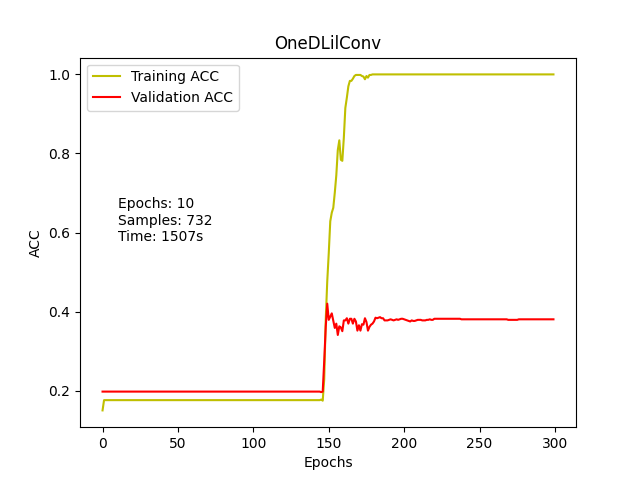
\includegraphics[height=5cm]{../../Plots/ba_plots/classnocascade/1dc.png}
    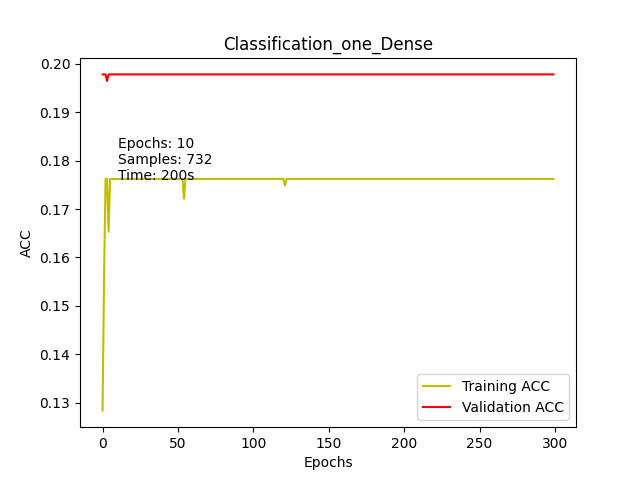
\includegraphics[height=5cm]{../../Plots/ba_plots/classnocascade/cod.png}
    \caption{\label{fig:nocascade} 
    \small{Die dargestellten Ergebnisse zeigen Testläufe ohne Kaskadierung. Konkret sind links die Resultate für das 1DC-Netzwerk (1DC:Comp/732//30) 
    und rechts für das COD-Netzwerk (COD:Comp/732//30) dargestellt. Es ist ersichtlich, dass eines der Modelle in einem lokalen Maximum stecken bleibt. 
    Zudem lässt sich aus den Ergebnissen ableiten, welcher maximale Accuracy-Wert unter der gegebenen, begrenzten Datenmenge realistischerweise 
    erreicht werden kann. Dieser Wert wird ausschließlich durch den Einsatz der vollständigen, hier beschriebenen Netzwerkarchitekturen erzielt.}}
\end{figure}

In Abbildung \ref{fig:nocascade} fällt auf, dass während der meisten Epochen kein Lerneffekt eintritt. Zudem ist Overfitting 
erkennbar – ein zu erwartendes Verhalten angesichts der geringen Menge an Trainingsdaten. Obwohl in diesem Experiment kein TF eingesetzt wurde, 
zeigt einer der beiden Plots in der Mitte einen plötzlichen Anstieg der Accuracy. Dieser Anstieg wurde durch eine minimale Verbesserung des 
Trainingswerts bei gleichzeitig minimaler Verschlechterung des Validierungswerts ausgelöst; beide Änderungen lagen im Bereich von 
Zehntelprozenten. Dies deutet auf das Erreichen eines lokalen Maximums im Trai-ningsverlauf hin.

Im Vergleich dazu bleibt das andere Netzwerk dauerhaft auf dem Niveau dieses lokalen Maximums – beide Resultate zeigen exakt identische Werte. 
Aus Abbildung \ref{fig:nocascade} lässt sich zudem ableiten, dass unter den gegebenen Bedingungen eine maximale Accuracy von etwa 40\% erreichbar 
ist. Dieser Wert stellt das globale Maximum dar, da er die bestmögliche Performanz auf den Trai-ningsdaten widerspiegelt.

Weder das reine Kaskadieren noch die Kombination aus Kaskadierung und TF erreichen vergleichbare Ergebnisse – beide Varianten 
erreichen lediglich eine maximale Accuracy von etwa 20\% und damit nur etwa die Hälfte der möglichen Leistung.

Diese Beobachtungen legen nahe, dass die Ursache für die stark eingeschränk-te Klassifikationsleistung im Direct-Cascade-Verfahren mit 
TF bereits in der Art der Kaskadierung selbst zu suchen ist. Mögliche Gründe hierfür könnten in der wiederholten Anwendung der 
Categorical-Crossentropy-Verlustfunktion liegen, die sich gegenseitig negativ beeinflussen könnte. Alternativ könnte auch die 
Softmax-Aktivierungsfunktion oder das konkrete Vorgehen beim Kaskadieren die Ursache darstellen.

Letztlich erweist sich der Einsatz von TF in Kombination mit dem Direct-Cascade-Verfahren unter Verwendung der in dieser Arbeit 
genutzten Datensätze und der beschriebenen Augmented Vectors als nicht zielführend, da die erzielten Accuracy-Werte selbst bei umfangreichen 
Trainingsdaten 60\% nicht über-schreiten und im Vergleich zu einem vollständig trainierten Netzwerk signifikant schlechter ausfallen.
